\documentclass[xcolor={dvipsnames}]{beamer}

\usetheme{default}
%\usetheme{Boadilla}
%\usetheme{Pittsburgh}

\usecolortheme{beaver}

\setbeamercovered{transparent}
\setbeamertemplate{navigation symbols}{} %remove navigation symbols

\usepackage[english]{babel}
\usepackage[latin1]{inputenc}
\usepackage{times}
\usepackage[T1]{fontenc}

\usepackage{tikz,amsmath,verbatim,wasysym}

\usepackage{animate}

\usepackage[normalem]{ulem}  % for "\sout" strikethrough

\newif\ifclipme\clipmetrue
\tikzset{labelstyle/.style={LabelStyle/.append style={#1}},linestyle/.style={LineStyle/.append style={#1}}}
\tikzset{LabelStyle/.initial={},LineStyle/.initial={}}

\newcommand{\mathWithDescription}[4][]{{%
    \tikzset{#1}%
    \tikz[baseline]{
        \node[draw=red,rounded corners,anchor=base] (m#4) {$\displaystyle#2$};
        \ifclipme\begin{pgfinterruptboundingbox}\fi
            \node[above of=m#4,font=\strut, LabelStyle] (l#4) {#3};
            \draw[-,red, LineStyle] (l#4) to (m#4);
        \ifclipme\end{pgfinterruptboundingbox}\fi
    }%
}}

\newcommand{\mathWithDescriptionStarred}[3][]{{%
    \clipmefalse%
    \mathWithDescription[#1]{#2}{#3}{\themathLabelNode}%
}}

\newcounter{mathLabelNode}

\newcommand{\mathLabelBox}[3][]{%
   \stepcounter{mathLabelNode}%
   \mathWithDescription[#1]{#2}{#3}{\themathLabelNode}%
   \vphantom{\mathWithDescriptionStarred[#1]{#2}{#3}{\themathLabelNode}}%
}


% math macros
\newcommand\bb{\mathbf{b}}
\newcommand\bbf{\mathbf{f}}
\newcommand\bn{\mathbf{n}}
\newcommand\bq{\mathbf{q}}
\newcommand\bs{\mathbf{s}}
\newcommand\bu{\mathbf{u}}
\newcommand\bv{\mathbf{v}}
\newcommand\bx{\mathbf{x}}
\newcommand\by{\mathbf{y}}
\newcommand\bz{\mathbf{z}}

\newcommand\bF{\mathbf{F}}
\newcommand\bQ{\mathbf{Q}}
\newcommand\bU{\mathbf{U}}
\newcommand\bV{\mathbf{V}}
\newcommand\bX{\mathbf{X}}

\newcommand\RR{\mathbb{R}}

\newcommand{\DDt}[1]{\ensuremath{\frac{d #1}{d t}}}
\newcommand{\ddt}[1]{\ensuremath{\frac{\partial #1}{\partial t}}}

\newcommand\Div{\nabla\cdot}
\newcommand\eps{\epsilon}
\newcommand\grad{\nabla}
\newcommand{\ip}[2]{\ensuremath{\left<#1,#2\right>}}


\title{Fluid layers, climates, and weak formulations}

\author{Ed Bueler}

\institute[UAF] % (optional, but mostly needed)
{
  Dept of Mathematics and Statistics, and Geophysical Institute\\
  University of Alaska Fairbanks \\
  \tiny (\emph{funded by NASA Modeling, Analysis, and Prediction program})%
}

\date{DMS Colloquium 5 April 2016}


\begin{document}
\graphicspath{{../domains/}{../obstacle/}{../cartoon/}{../refinemass/}{../../images/}{../../../talks-public/commonfigs/}{../../../sia-fve/talks/}}

\begin{frame}
  \titlepage
\end{frame}


\begin{frame}{my motivation for this topic}
\begin{itemize}
\item gradual realization, during sabbatical last year:
\begin{center}
\alert{there is a whole class of climate modeling problems which people are doing the wrong way}
\end{center}
  \begin{itemize}
  \item[$\circ$] ``people'' = scientists/modelers who study cryosphere
  \item[$\circ$] concern: choice of mathematical formulation
  \end{itemize}
\visible<2>{

\bigskip
\item i.e.~watch me tilt at windmills
}
\end{itemize}

\visible<2>{
\begin{center}
\includegraphics[width=0.5\textwidth,keepaspectratio=true]{quixotewindmills}
\end{center}
}
\end{frame}


\begin{frame}{outline}
  \tableofcontents
\end{frame}


\section{glaciers and ice sheets}

\begin{frame}{glaciers and ice sheets}

\begin{columns}
\begin{column}{0.45\textwidth}
\begin{itemize}
\small
\item they move (flow and slide) under their own weight
  \begin{itemize}
  \scriptsize
  \item[$\circ$] speed $1$ cm/yr -- $10$ km/yr
  \item[$\circ$] geometry determined in part by flow
  \end{itemize}
\small
\item they accumulate snow, or melt, as sensitive function of global climate
  \begin{itemize}
  \scriptsize
  \item[$\circ$] Canadians should be grateful
  \end{itemize}
\small
\item ice sheet = big glacier
\small
\item about 66 m (= 215 ft) of sea level rise equivalent
  \begin{itemize}
  \scriptsize
  \item[$\circ$] Antarctic ice sheet $=$ 60 m
  \item[$\circ$] Greenland ice sheet $=$ 6m
  \item[$\circ$] Alaska's glaciers $<$ 0.5 m
  \end{itemize}
\end{itemize}
\end{column}
\begin{column}{0.55\textwidth}
\includegraphics[width=\textwidth,keepaspectratio=true]{polaris}

\includegraphics[width=\textwidth,keepaspectratio=true]{mass-bal-atmos}
\end{column}
\end{columns}
\end{frame}


\begin{frame}{glacier model paradigms}

\begin{itemize}
\item<1-2> glacier problem \alert<1-2>{(to most numerical modelers)}:
   \begin{quote}
   given geometry of glacier, and stress boundary conditions, determine velocity of ice
   \end{quote}
\vspace{-4mm}
  \begin{itemize}
  \item<2>[$\circ$] a slow flow ($\operatorname{Re} \ll 1$) allows you to think this way
  \end{itemize}

\bigskip
\item<3> glacier problem \alert<3>{(to most actual glaciologists)}:
   \begin{quote}
   given climate and topography, determine glaciated area and thicknesses of glaciers
   \end{quote}
\end{itemize}
\end{frame}


\begin{frame}{glacier notation}

\begin{center}
\includegraphics[width=0.5\textwidth,keepaspectratio=true]{groundedscheme}
\end{center}

\begin{itemize}
\item unknowns:
  \begin{itemize}
  \item[$\circ$]  $h(t,x,y)$ ice thickness \hfill \dots also $s=h+b$ surface elevation
  \item[$\circ$]  $\bU(t,x,y,z) = \left<u,v,w\right>$ ice velocity
  \end{itemize}
\item \only<1>{data}\only<2>{\alert{uncertain ``data'' from other models}}:
  \begin{itemize}
  \item[$\circ$]  $b(x,y)$ bed elevation \only<2>{\quad \alert{\dots improving for ice sheets}}
  \item[$\circ$]  $a(t,x,y,z)$ surface mass balance  \only<2>{\quad \alert{\dots from GCM}}
    \begin{itemize}
    \item a.k.a.~accumulation/ablation function
    \item $a=$ precipitation $-$ melt
    \end{itemize}
  \end{itemize}
\item ignored in this talk:
  \begin{itemize}
  \item[$\circ$]  conservation of energy (temperature/enthalpy)
  \item[$\circ$]  floating ice
  \end{itemize}
\end{itemize}
\end{frame}


\begin{frame}{models solve coupled conservation equations}

\begin{columns}
\begin{column}{0.7\textwidth}
\begin{itemize}
\small
\item \emph{mass conservation}
\begin{equation*}
h_t + \Div\bq = a
\end{equation*}
    \begin{itemize}
    \footnotesize
    \vspace{-5mm}
    \item[$\circ$] in ice-covered set $I_t = \{h>0\} \subset \RR^2$
        \begin{itemize}
        \item changes in time
        \item climate $a$ and bed $b$ defined on $\Omega\subset \RR^2$ s.t.~$I_t\subset\Omega$
        \end{itemize}
    \item[$\circ$] $\bq=\bq[\bU,h]$ is ice flux
        \begin{itemize}
        \item vertically-integrated
        \end{itemize} 
    \end{itemize}
\item \emph{momentum conservation}
\begin{equation*}
  \nabla \cdot \bU = 0 \quad \text{and} \quad - \nabla \cdot \tau_{ij} + \nabla p - \rho\, \mathbf{g} = 0
\end{equation*}
    \begin{itemize}
    \footnotesize
    \vspace{-5mm}
    \item[$\circ$] in $E_t \subset \RR^3$; changes in time
        \begin{itemize}
        \item $I_t = \Pi_z E_t$
        \end{itemize}
    \item[$\circ$] incompressible power-law Stokes
        \begin{itemize}
        \item $D_{ij} = A \tau^{2} \tau_{ij}$
        \end{itemize}
    \item[$\circ$] geometry ($h$ \& $b$) enters into b.c.s
    \end{itemize}
\end{itemize}
\end{column}
\begin{column}{0.3\textwidth}
\includegraphics[width=1.1\textwidth,keepaspectratio=true]{domainfig}

\vspace{0.5in}
\includegraphics[width=1.0\textwidth,keepaspectratio=true]{polaris}
\end{column}
\end{columns}
\end{frame}


\begin{frame}{many possible momentum equations}

  \begin{itemize}
  \scriptsize
  \item[$\circ$] incompressible Stokes
\begin{equation*}
  \nabla \cdot \bU = 0 \qquad \text{and} \qquad - \nabla \cdot \tau_{ij} + \nabla p - \rho\, \mathbf{g} = 0
\end{equation*}
  \item[$\circ$] Blatter-Pattyn equations [$\eta$ is effective viscosity]
$$-\Div \left[\eta \begin{pmatrix}
4 u_x+2v_y & u_y+v_x   & u_z \\
u_y+v_x    & 2u_x+4v_y & v_z
\end{pmatrix} \right] + \rho g \grad s = 0$$
  \item[$\circ$] shallow shelf approximation (SSA)
$$-\Div \left[\bar \eta h \begin{pmatrix}
4 \bar u_x+2\bar v_y & \bar u_y+\bar v_x   \\
\bar u_y+\bar v_x    & 2\bar u_x+4\bar v_y
\end{pmatrix} \right] - \tau_b + \rho g h \grad s = 0$$
  \item[$\circ$] non-sliding shallow ice approximation (SIA)
$$-\frac{\partial}{\partial z} \left[\eta \begin{pmatrix}
u_z \\
v_z
\end{pmatrix} \right] + \rho g \grad s = 0
\qquad \to \qquad
\ip{\bar u}{\bar v} = -\Gamma h^{\nu+2} |\grad s|^{\nu-1} \grad s$$
  \end{itemize}

\begin{itemize}
\item slow-fluid momentum-conservation models always
\begin{center}
\alert{generate velocity $\bU=\left<u,v,w\right>$ from geometry $h$ \& $b$}
\end{center}
\item abstract momentum equations: \qquad $\mathcal{M}(\bU,h,b)=0$
\end{itemize}
\end{frame}


\begin{frame}{toward better models}

\begin{itemize}
\item abstracted model of glaciers:
\begin{align*}
h_t + \Div\bq &= a \qquad \text{in } I_t = \{h>0\} \subset \RR^2 \\
\mathcal{M}(\bU,h,b) &= 0 \qquad \text{in } E_t \subset \RR^3 \\
\bU &= \left<u,v,w\right> \\
\bq &= \int_b^{h+b} \left<u,v\right>\,dz
\end{align*}

\medskip
\item \emph{my goal}: better numerical glacier models
  \begin{itemize}
  \item[$\circ$] effective for long runs ($\sim 100$ ka) at high res ($\sim 1$ km) \only<2-3>{\hfill\alert{\large\frownie{}}}
  \item[$\circ$] without first-order time-splitting errors \only<2-3>{\hfill\alert{\large\frownie{}}}
  \item[$\circ$] without explicit time-step restrictions \only<2-3>{\hfill\alert{\large\frownie{}}}
  \end{itemize}
\visible<2-3>{\item \alert{vs PISM = Parallel Ice Sheet Model, \texttt{pism-docs.org}}}

\medskip
\visible<3>{\item mathematical model at top is not good enough}
\end{itemize}
\end{frame}


\begin{frame}{practical numerical modeling}

\begin{itemize}
\small
\item some limitations in our big ice sheet model PISM:
  \begin{itemize}
  \item[$\circ$] explicit time-stepping
  \item[$\circ$] free boundary by truncation
  \end{itemize}
\item challenge: flowing ice (e.g.~Greenland) is nearly-fractal
\end{itemize}

\begin{center}
\includegraphics[height=5.2cm,keepaspectratio=true]{Greenland_thinning} \quad \includegraphics[height=5.2cm,keepaspectratio=true]{ice-mask-900m}
\end{center}
\end{frame}


\AtBeginSection[] % Do nothing for \section*
{
\begin{frame}<beamer>
\frametitle{outline}
\tableofcontents[currentsection]
\end{frame}
}

\section{generalize to fluid layers and their climates}

\begin{frame}{a fluid layer}

\begin{center}
\includegraphics[width=0.7\textwidth,keepaspectratio=true]{cartoon-wclimate}
\end{center}

\vspace{-7mm}
\begin{itemize}
\item mass conservation eqn applies to broader class:
  \begin{center}
  \alert{a fluid layer on a substrate, evolving in a climate}
  \end{center}
\item mass conservation PDE:
\begin{equation*}
h_t + \Div\bq = {\color{blue} a}
\end{equation*}
    \begin{itemize}
    \vspace{-4mm}
    \item[$\circ$] $h$ is a thickness so $h\ge 0$
    \item[$\circ$] signed source ${\color{blue} a}$ is the ``climate''; ${\color{blue} a}>0$ shown downward
    \item[$\circ$] hidden, but important, part of the model: $\bq=\bq[h,b]$
    \item[$\circ$] \alert{PDE applies only where $h>0$}
    \end{itemize}
\end{itemize}
\end{frame}


\begin{frame}{fluid layers: \emph{the troubles}}

\vspace{-1.2mm}

\begin{center}
\only<1>{\includegraphics[width=0.95\textwidth,keepaspectratio=true]{cartoon-sensitive-three}}
\only<2>{\includegraphics[width=0.95\textwidth,keepaspectratio=true]{cartoon-sensitive-one}}
\only<3>{\includegraphics[width=0.95\textwidth,keepaspectratio=true]{cartoon-sensitive-two}}
\end{center}

\vspace{-16mm}
$$h_t + \Div\bq = a$$

  \begin{itemize}
  \item<1-> $h=0$ \emph{and what else} at \alert<1>{free boundary}?
     \begin{itemize}
     \item<1->[$\circ$] geometry at free boundary depends on both $\bq$ and $a$
     \end{itemize}
  \item<2-> $a<0$ not ``detected'' by model where $h=0$
     \begin{itemize}
     \item<2->[$\circ$] how to do mass conservation accounting \alert<2>{here}?
     \end{itemize}
  \item<3> $a\approx 0$ sensitive-threshold behavior
     \begin{itemize}
     \item<3>[$\circ$] nucleate new fluid model \alert<3>{here} if $a<0$ switches to $a>0$
     \end{itemize}
  \end{itemize}
\end{frame}


\begin{frame}{actual glacier free boundary}

\begin{center}
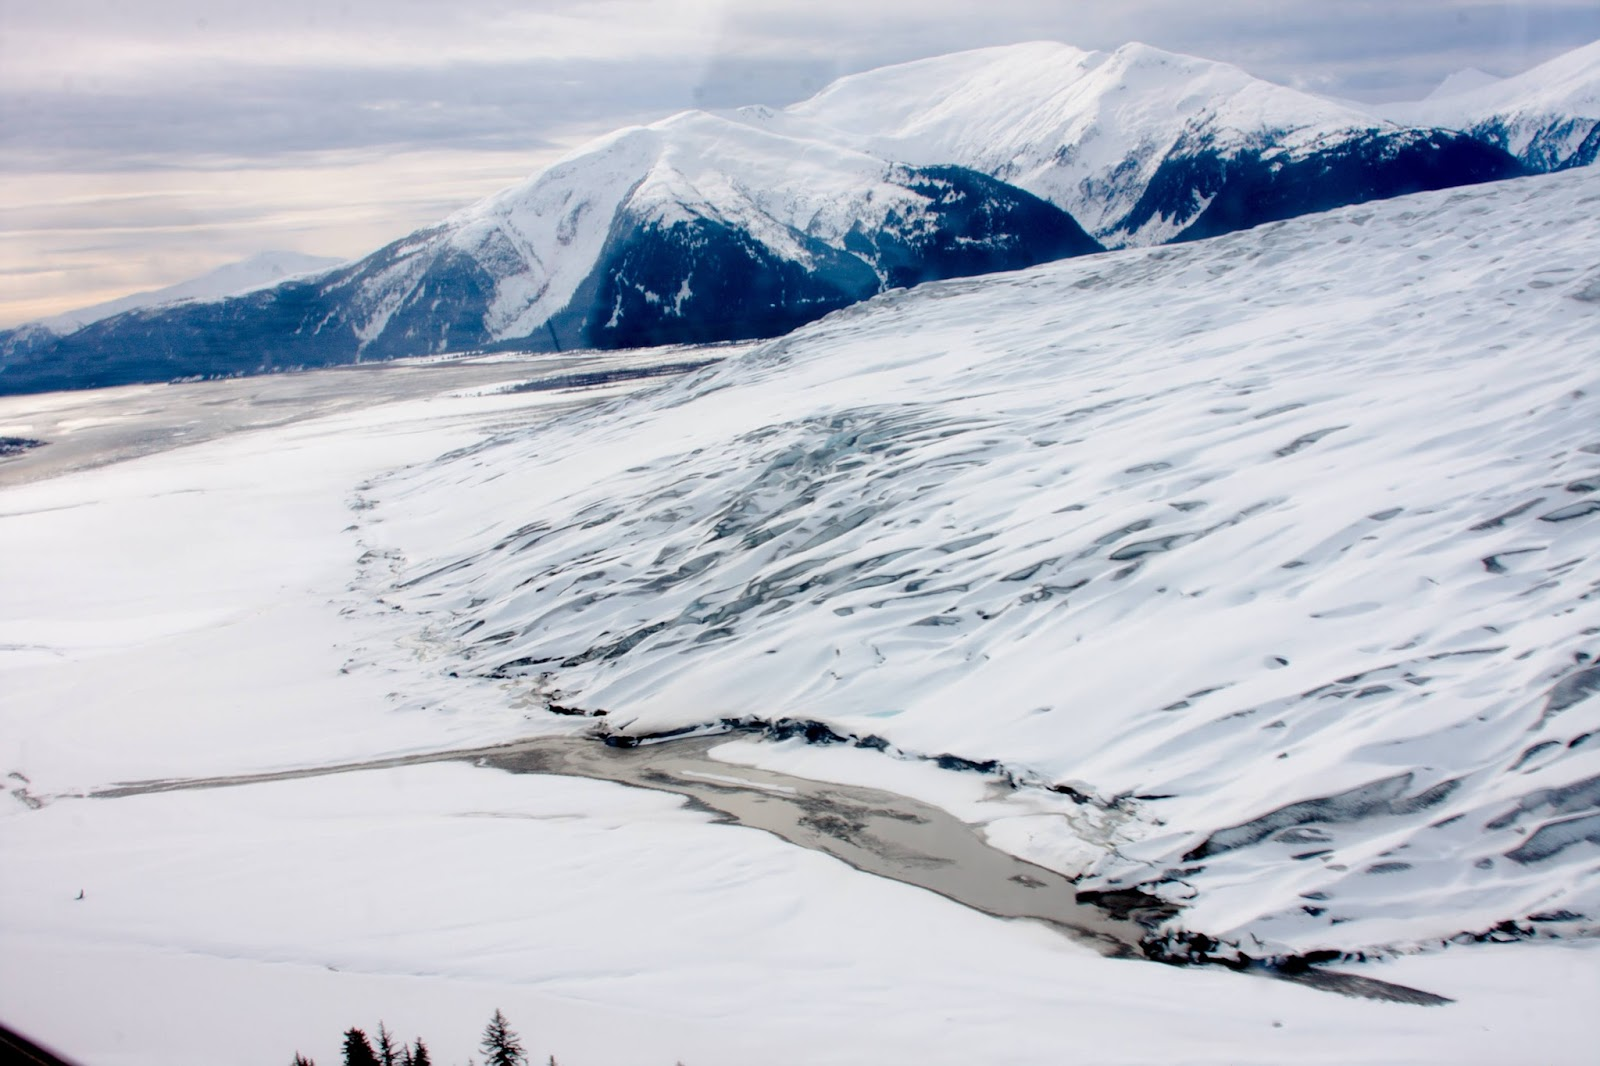
\includegraphics[width=0.95\textwidth,keepaspectratio=true]{truffertaku2016}
\end{center}

\tiny \hfill Martin Truffer, Taku Glacier SE Alaska, March 2016
\end{frame}


\begin{frame}{examples: fluid layers in climates}

\includegraphics[width=0.4\textwidth,keepaspectratio=true]{polaris}
\hfill
\includegraphics[width=0.45\textwidth,keepaspectratio=true]{supp4rignot-small}

\small glaciers \& ice sheets \hfill sea ice

\medskip
\includegraphics[width=0.33\textwidth,keepaspectratio=true]{marsh-water}
\quad \includegraphics[width=0.33\textwidth,keepaspectratio=true]{tsunami-sendai}
\quad \includegraphics[width=0.27\textwidth,keepaspectratio=true]{aral-sea-1964-2014}

\small tidewater marsh \hfill tsunami inundation \hfill \phantom{foo} Aral Sea\,
\end{frame}


\begin{frame}{time scales for major geometry changes}

\begin{tabular}{rcc}
 & \emph{lateral transport} & \emph{accumulation/ablation} \\ \hline
\alert<2>{glacier/ice sheet} & \alert<2>{100 years} & \alert<2>{100 years} \\
\alert<2>{sea ice} & \alert<2>{1 week?} & \alert<2>{1 month?} \\ \hline
\alert<2>{tidewater marsh} & \alert<2>{1 hour} & \alert<2>{1 day?} \\
\only<1>{tsunami & 10 seconds & 1 year \\}
\only<2>{\sout{tsunami} & \sout{10 seconds} & \sout{1 year} \\}
\only<1>{Aral Sea & ? & 1 year \\}
\only<2>{\sout{Aral Sea} & \sout{?} & \sout{1 year}}
\end{tabular}

\bigskip

\begin{itemize}
\item consider time-scales for major changes in geometry of the fluid layer from two sources:
   \begin{itemize}
   \item[$\circ$] motion of the fluid from forces applied at boundary (or body forces); \emph{lateral transport}
   \item[$\circ$] \emph{accumulation} (e.g.~precipitation or aggregation) and \emph{ablation} (melting, evaporation, sublimation)
   \end{itemize}

\medskip
\item<2> \alert<2>{this talk}: cases where these time-scales are comparable
\end{itemize}
\end{frame}


\begin{frame}{case: tsunamis}

\begin{center}
\includegraphics[width=0.9\textwidth,keepaspectratio=true]{tsunami-sendai}
\end{center}

\begin{itemize}
\item flux $\bq$ dominates \dots climate $a$ irrelevant
\end{itemize}
\end{frame}


\begin{frame}{case: Aral Sea on  Kazakhstan/Uzbekistan border}

\begin{center}
\includegraphics[width=0.65\textwidth,keepaspectratio=true]{aral-sea-1964-2014}
\end{center}

\begin{itemize}
\item top row: 1964, 1989, 1995?
\item bottom row: 1999, 2002?, 2014
\item climate $a$, and bdry fluxes, dominate \dots flux $\bq$ irrelevant
\end{itemize}
\end{frame}


\begin{frame}{fluid layers in climates: my actual examples}

\includegraphics[width=0.4\textwidth,keepaspectratio=true]{polaris}
\hfill
\includegraphics[width=0.45\textwidth,keepaspectratio=true]{supp4rignot-small}

\small glaciers \& ice sheets $\checkmark$ \hfill sea ice $\checkmark$

\medskip
\begin{center}
\includegraphics[width=0.25\textwidth,keepaspectratio=true]{marsh-water}

\small tidewater marsh ?
\end{center}
\end{frame}


\begin{frame}{anyone numerically modeled this situation before?}

\vspace{-2mm}

\begin{itemize}
\item yes, of course!  generic results:
    \begin{itemize}
    \item[$\circ$] \emph{ad hoc} schemes near the free boundary
    \item[$\circ$] only numerics; almost no continuum modeling
    \end{itemize}
\end{itemize}

\medskip
\begin{columns}
\begin{column}{0.45\textwidth}
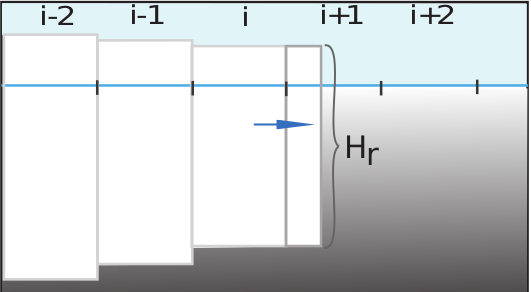
\includegraphics[width=0.7\textwidth,keepaspectratio=true]{Albrechtetal2011half}

\scriptsize volume-of-fluid method at ice shelf fronts

\tiny (Albrecht et al, 2011)

\medskip
\includegraphics[width=0.45\textwidth,keepaspectratio=true]{JaroschSchoofAnslow2013}

\scriptsize glacier ice on steep terrain

\smallskip
\tiny (Jarosch, Schoof, Anslow, 2013)
\end{column}

\begin{column}{0.5\textwidth}
\hfill 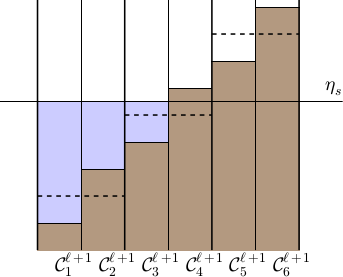
\includegraphics[width=0.45\textwidth,keepaspectratio=true]{LeVequeGeorgeBerger2011}

\hfill \scriptsize tsunami run-up on shore

\smallskip
\hfill \tiny (LeVeque, George, Berger, 2011)

\medskip
\hfill \includegraphics[width=0.55\textwidth,keepaspectratio=true]{jouvet-two-grids}

\hfill \scriptsize volume-of-fluid method at glacier surface

\hfill \tiny (Jouvet et al 2008)
\end{column}
\end{columns}
\end{frame}


\section{weak formulations}

\begin{frame}{nonlinear complementarity problems (NCP)}

\begin{itemize}
\item given differentiable $\bF:\RR^n \to \RR^n$, the NCP seeks $\bz\in\RR^n$ s.t.
\begin{equation*}
\bz \ge 0, \quad \bF(\bz) \ge 0, \quad \bz^\top \bF(\bz) = 0
\end{equation*}
\end{itemize}
\end{frame}


\begin{frame}{example NCP}

\begin{columns}
\begin{column}{0.5\textwidth}
\begin{itemize}
\small
\item \alert{1d obstacle problem}: given $\psi(x)$, find $u(x)$ so that 
   $$u(x) \ge \psi(x)$$
and
   $$-u''(x) = 0 \quad \text{where } u>\psi$$
\item discretize \dots
\item note $-u''\ge 0$ \dots and think about the gap \dots
\item in NCP form:
\begin{align*}
{\color{red} z_j} &= u_j - \psi_j \ge 0\\
{\color{ForestGreen} F_j}(\bz) &= - \frac{z_{j+1} - 2 z_j + z_{j-1}}{\Delta x^2} - \psi_j'' \ge 0 \\
\sum_j &{\color{red} z_j} {\color{ForestGreen} F_j}(\bz) = 0
\end{align*}
\end{itemize}
\end{column}
\begin{column}{0.5\textwidth}
\includegraphics[width=1.05\textwidth,keepaspectratio=true]{obstacle1d}

\medskip
\includegraphics[width=1.05\textwidth,keepaspectratio=true]{vi1d}

\medskip
\includegraphics[width=1.05\textwidth,keepaspectratio=true]{ncp1d}
\end{column}
\end{columns}
\end{frame}


\begin{frame}{variational inequalities (VI)}

\begin{itemize}
\item more general than NCP
\item suppose $\mathcal{K}\subseteq \RR^n$ is convex and closed
\item given differentiable $\bF:\RR^n \to \RR^n$, the VI seeks $\bu\in\mathcal{K}$ s.t.
\begin{equation*}
     \ip{\bF(\bu)}{\bv-\bu} \ge 0 \qquad \forall \bv \in \mathcal{K}
\end{equation*}
\item also makes sense in $\infty$ dimensions
\end{itemize}

\begin{columns}
\begin{column}{0.4\textwidth}
\small
\begin{itemize}
\item \alert{1d obstacle problem}:
  $$\mathcal{K} = \{{\color{red} u_j} \ge {\color{blue} \psi_j}\}$$
  $$F_j(\bu) = - \frac{u_{j+1} - 2 u_j + u_{j-1}}{\Delta x^2}$$
\end{itemize}
\end{column}
\begin{column}{0.6\textwidth}
\includegraphics[width=\textwidth,keepaspectratio=true]{vi1d}
\end{column}
\end{columns}
\end{frame}


\begin{frame}{NCP/VI generalities}

\begin{itemize}
\item suppose $\mathcal{K}\subseteq \RR^n$ is a cone (always in this talk)
\item then
\begin{center}
\alert{NCP $\iff$ VI}
\end{center}
\item both formulations
  \begin{itemize}
  \item[$\circ$]  generalize nonlinear eqns $\bF(\bx)=0$ to allow constraints
  \item[$\circ$]  are nonlinear, even if $\bF$ is linear or affine
  \item[$\circ$]  in practice: need iterative approach to solve
  \end{itemize}
\item (convex optimization) $\implies$ VI $\iff$ NCP
  \begin{itemize}
  \item[$\circ$]  i.e.~find minimum of $\Phi[\bz]$ from $\mathcal{K}$
  \item[$\circ$]  symmetric Jacobian/Hessian ($\bF' = \Phi''$)
  \item[$\circ$]  \emph{but}: NCP/VI arising in fluid layer problems are never optimizations (to my knowledge)
  \end{itemize}
\end{itemize}
\end{frame}


\newcommand{\singletsmc}{\frac{h^\ell - h^{\ell-1}}{\Delta t} + \Div \bq^\ell = a^\ell}


\begin{frame}{semi-discretize in time}

\begin{itemize}
\item back to our fluid layer coupled model \dots
\item from now on: assume $\bq=0$ on any open set where $h=0$
    \begin{itemize}
    \item[$\circ$] because it is a flowing \emph{layer}
    \end{itemize}
\item semi-discretize:
$$\begin{matrix}
 h_t + \Div\bq = a \\
 \phantom{foo} \\
 \mathcal{M}(\bU,h,b) = 0
\end{matrix} \qquad \to \qquad \begin{matrix}
 \singletsmc \\
 \phantom{foo} \\
 \mathcal{M}(\bU^\ell,h^\ell,b) = 0
\end{matrix}$$
        \begin{itemize}
        \item[$\circ$] $h^\ell(x,y) \approx h(t^\ell,x,y)$
        \item[$\circ$] coupling through $\bq=\bq(\bU,h)$
        \end{itemize}
\item this is still a continuum problem (in space)
\item details of flux $\bq^\ell$ and source $a^\ell$ come from scheme
        \begin{itemize}
        \item[$\circ$] backward-Euler shown
        \item[$\circ$] could use other $\theta$-methods or BDFs
        \end{itemize}
\end{itemize}
\end{frame}


\begin{frame}{mass conservation: strong form \dots is inadequate}

\begin{itemize}
\item single time-step mass conservation equation
\begin{equation}
\singletsmc \tag{MC} \label{mc}
\end{equation}
    \begin{itemize}
    \item[$\circ$] \emph{strong form} of (MC)
    \end{itemize}

\bigskip
\item \alert{need to weakly-pose (MC), incorporating $h^\ell\ge 0$ constraint}
    \begin{itemize}
    \item[$\circ$] seek $h^\ell(x,y)$ and location of the free boundary simultaneously
    \end{itemize}
\end{itemize}
\end{frame}


\begin{frame}{mass conservation: VI form}

\begin{itemize}
\item first weak formulations of \eqref{mc} for glaciers were VIs
    \begin{itemize}
    \item[$\circ$] Calvo et al (2002): 1d glacier on flat bed
    \item[$\circ$] Jouvet \& Bueler (2012): 2d glacier on general bed
    \end{itemize}
\item define $\mathcal{K} = \left\{v \in W^{1,p}(\Omega) \,\Big|\, v\ge 0\right\}$
\item VI form of \eqref{mc}: \quad find $h^\ell\in\mathcal{K}$ s.t.
    $$\int_\Omega h^\ell (v - h^\ell) - \Delta t\, \bq^\ell \cdot \grad(v - h^\ell) \ge \int_\Omega \left(h^{\ell-1} + \Delta t\, a^\ell\right) (v - h^\ell)$$
for all $v \in \mathcal{K}$
    \begin{itemize}
    \item[$\circ$] derive from strong form \eqref{mc} by integration-by-parts plus thoughts about $h^\ell=0$ areas
    \end{itemize}
\end{itemize}
\end{frame}


\begin{frame}{mass conservation: NCP form}

\begin{itemize}
\item define
    $$F(h) = h - h^{\ell-1} + \Delta t\, \Div \bq - \Delta t\, a$$
\item NCP form of \eqref{mc}: \quad find $h^\ell$ s.t.
   $$h^\ell \ge 0, \quad F(h^\ell) \ge 0, \quad h^\ell F(h^\ell) = 0$$
\item setwise statements from the NCP:
    \begin{itemize}
    \item[$\circ$] where $h^\ell > 0$,
        $$F(h^\ell) = 0 \qquad \iff \qquad \text{strong form \eqref{mc}}$$
        \vspace{-4mm}
        \begin{itemize}
        \item interior condition
        \end{itemize}
    \item[$\circ$] where $h^\ell = 0$,
        $$h^{\ell-1} + \Delta t\, a^\ell \le 0$$
        \vspace{-4mm}
        \begin{itemize}
        \item says ``climate is sufficiently negative to remove old thickness'' (during the time step)
        \end{itemize}
    \end{itemize}
\end{itemize}
\end{frame}


\begin{frame}{numerical solution of the weak problem}

for weak formulation (NCP or VI) of \eqref{mc}:
\begin{itemize}
\item can be solved by a Newton method modified for constraint
\item scalable \& parallel implementations in C are in PETSc$^*$
  \begin{itemize}
  \item[$\circ$]  RS and SS methods for NCP (next slide)
  \end{itemize}
\end{itemize}

\vspace{15mm}
{\scriptsize $^*$Portable Extensible Toolkit for Scientific computation, \texttt{www.mcs.anl.gov/petsc}}
\end{frame}


\begin{frame}{constrained-Newton algorithms}

two Newton line search NCP methods:
\begin{itemize}
\item  ``reduced-space'' = \alert{RS}
    \begin{itemize}
    \item[$\circ$] inactive set $\mathcal{I} = \{i \,:\, z_i > 0 \text{ or } F_i(\bz) \le 0\}$
    \item[$\circ$] \emph{algorithm}: compute Newton step $\bs^k$ by
     $$\big[J(\bz^k)\big]_{\mathcal{I}^k,\mathcal{I}^k} \bs_{\mathcal{I}^k} = - \bF_{\mathcal{I}^k}(\bz^k)$$
     then do projected ($\{\bz\ge 0\}$) line search
    \end{itemize}
\item  ``semi-smooth'' = \alert{SS}
    \begin{itemize}
    \item[$\circ$] choose ``NCP function'':
\vspace{-2mm}
    $$\phi(a,b)=0 \quad \iff \quad a\ge 0, b\ge 0, ab=0$$
    \item[$\circ$] \emph{algorithm}: compute Newton step $\bs^k$ by
    $$L^k \bs^k = - \phi(\bz^k,\bF^k(\bz^k))$$
    where $L^k$ is element of $\partial_B \phi(\bz^k,\bF^k(\bz^k))$; then do line search
    \end{itemize}
\end{itemize}
\end{frame}


\begin{frame}{1D time-stepping movies (and $\bq$ flexibility)}

\begin{columns}
\begin{column}{0.35\textwidth}
\alert{same:}

\begin{itemize}
\scriptsize
\item equation \eqref{mc}
\item BEuler time-step
\item climate $a$
\item bed shape $b$
\item constraint-respecting

Newton scheme
\end{itemize}

\vspace{2mm}

\alert{top:}

\scriptsize

\medskip
$\bq = v_0 h$

hyperbolic advection with

constant velocity

\vspace{5mm}

\normalsize 

\alert{bottom:}

\scriptsize

\medskip
$\bq = - \Gamma |h|^{n+2}$

$\phantom{\bq = }\, \cdot |\grad s|^2 \grad s$

nonlinear degenerate

diffusion
\end{column}
\begin{column}{0.5\textwidth}
\hspace{-15mm}
\animategraphics[autoplay,loop,height=3.0cm]{6}{../anim/adv/u-}{1}{50}

\bigskip
\hspace{-15mm}
\animategraphics[autoplay,loop,height=3.0cm]{6}{../anim/sia/u-}{1}{50}

\end{column}
\end{columns}
\end{frame}


\begin{frame}{finite volume element (FVE) discretization}

\begin{itemize}
\item thickness $h(x,y)$ lives in $Q^1$ FEM space $\subset W^{1,p}(\Omega)$
    \begin{itemize}
    \item[$\circ$] $h$ is bilinear on elements $\square_{j,k}$
    \end{itemize}
\item (MC) discretized to control-volume integral on $V=V_{j,k}$
\item in steady case ($\Delta t = \infty$) it looks like
    $$\Div \bq = a \qquad \to \qquad \int_{\partial V} \bq \cdot \bn \,ds \stackrel{\ast}{=} \int_V a \,dx\,dy$$ 
    \begin{itemize}
    \vspace{-2mm}
    \item[$\circ$] $\Delta t=\infty$ is the hard case for numerics
    \end{itemize}

\smallskip
\item an FVE method is an FEM where $\ast$ is the weak form
    \begin{itemize}
    \item[$\circ$] \emph{equiv}: Petrov-Galerkin FEM with $1_V$ as test function
    \item[$\circ$] no symmetry in weak form (\dots no loss for known cases)
    \end{itemize}
\end{itemize}

\begin{center}
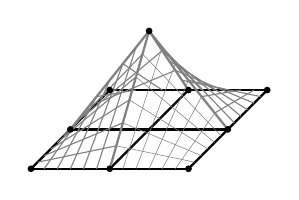
\begin{tikzpicture}[scale=0.25]
  % strong grid around elements
  \draw[thick] (0,0) -- (8,0);
  \draw[thick] (2,2) -- (10,2);
  \draw[thick] (4,4) -- (12,4);
  \draw[thick] (0,0) -- (4,4);
  \draw[thick] (4,0) -- (8,4);
  \draw[thick] (8,0) -- (12,4);

  \def\ytop{7};

  % tent lines
  \draw[gray,thick] (6,\ytop) -- (4,0);
  \draw[gray,thick] (6,\ytop) -- (2,2);
  \draw[gray,thick] (6,\ytop) -- (10,2);
  \draw[gray,thick] (6,\ytop) -- (8,4);

  \def\dx{(10.0-6.0)/6};
  \def\dy{(2.0-\ytop)/6};
  \foreach \jj in {1,...,5}
  {
       \draw[gray,very thin] ({6+\jj*\dx},{\ytop+\jj*\dy}) -- ({4+(4/6)*\jj},0.0);
  }

  \def\dx{(4.0-6.0)/6};
  \def\dy{(0.0-\ytop)/6};
  \foreach \jj in {1,...,5}
  {
       \draw[gray,very thin] ({6+\jj*\dx},{\ytop+\jj*\dy}) -- ({10-(2/6)*\jj},{2-(2/6)*\jj});
  }

  \def\dx{(2.0-6.0)/6};
  \def\dy{(2.0-\ytop)/6};
  \foreach \jj in {1,...,5}
  {
       \draw[gray,thin] ({6+\jj*\dx},{\ytop+\jj*\dy}) -- ({4-(4/6)*\jj},0.0);
  }

  \def\dx{(4.0-6.0)/6};
  \def\dy{(0.0-\ytop)/6};
  \foreach \jj in {1,...,5}
  {
       \draw[gray,thin] ({6+\jj*\dx},{\ytop+\jj*\dy}) -- ({2-(2/6)*\jj},{2-(2/6)*\jj});
  }

  \def\dx{(10.0-6.0)/6};
  \def\dy{(2.0-\ytop)/6};
  \foreach \jj in {1,...,5}
  {
       \draw[gray,thin] ({6+\jj*\dx},{\ytop+\jj*\dy}) -- ({8+(4/6)*\jj},4.0);
  }

  \def\dx{(8.0-6.0)/6};
  \def\dy{(4.0-\ytop)/6};
  \foreach \jj in {1,...,5}
  {
       \draw[gray,thin] ({6+\jj*\dx},{\ytop+\jj*\dy}) -- ({10+(2/6)*\jj},{2+(2/6)*\jj});
  }

  \def\dx{(2.0-6.0)/3};
  \def\dy{(2.0-\ytop)/3};
  \foreach \jj in {1,...,2}  % reduce clutter
  {
       \draw[gray,thin] ({6+\jj*\dx},{\ytop+\jj*\dy}) -- ({8-(4/3)*\jj},4.0);
  }

  \def\dx{(8.0-6.0)/3};
  \def\dy{(4.0-\ytop)/3};
  \foreach \jj in {1,...,2}
  {
       \draw[gray,thin] ({6+\jj*\dx},{\ytop+\jj*\dy}) -- ({2+(2/3)*\jj},{2+(2/3)*\jj});
  }

  % nodes in base plane
  \filldraw (0,0) circle (4pt);
  \filldraw (4,0) circle (4pt);
  \filldraw (8,0) circle (4pt);
  \filldraw (2,2) circle (4pt);
  %\filldraw (6,2) circle (4pt);   % (x_j,y_k) is at (6,2)
  \filldraw (10,2) circle (4pt);
  \filldraw (4,4) circle (4pt);
  \filldraw (8,4) circle (4pt);
  \filldraw (12,4) circle (4pt);

  % node at tent top
  \filldraw (6,\ytop) circle (4pt);
\end{tikzpicture}
\qquad \qquad
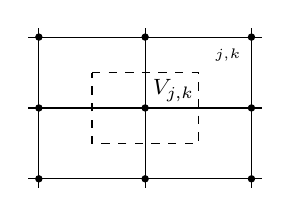
\begin{tikzpicture}[scale=0.45]
  % strong grid around elements
  \draw (-0.3,0) -- (6.3,0);
  \draw (-0.3,2) -- (6.3,2);
  \draw (-0.3,4) -- (6.3,4);
  \draw (0,-0.25) -- (0,4.25);
  \draw (3,-0.25) -- (3,4.25);
  \draw (6,-0.25) -- (6,4.25);
  % nodes
  \filldraw (0,0) circle (2.5pt);
  \filldraw (3,0) circle (2.5pt);
  \filldraw (6,0) circle (2.5pt);
  \filldraw (0,2) circle (2.5pt);
  \filldraw (3,2) circle (2.5pt);
  \filldraw (6,2) circle (2.5pt);
  \filldraw (0,4) circle (2.5pt);
  \filldraw (3,4) circle (2.5pt);
  \filldraw (6,4) circle (2.5pt);
  % outline control volume
  \draw[dashed] (1.5,3) -- (4.5,3) -- (4.5,1) -- (1.5,1) -- cycle;
  % label elements and control volume
  \draw (3.8,2.5) node {\footnotesize $V_{j,k}$};
  \draw (5.35,3.5) node {\scriptsize $\square_{j,k}$};
\end{tikzpicture}
\end{center}
\end{frame}


\begin{frame}{restrict to shallow ice approximation (SIA) for glaciers}

\begin{itemize}
\item from now on, restrict to nonsliding SIA:
    $$\bq = - \Gamma h^{\nu+2} |\grad s|^{\nu-1} \grad s$$

    \begin{itemize}
    \item[$\circ$] where $s=h+b$
    \item[$\circ$] justified by small-aspect-ratio argument
    \end{itemize}
\end{itemize}
\end{frame}


\begin{frame}{glacier numerics: quadrature and upwinding}

\begin{itemize}
\item FD scheme for SIA fits into above FVE framework
  \begin{itemize}
  \item[$\circ$] i.e.~Mahaffy (1976) \dots but it has weird quadrature
  \item[$\circ$] improved convergence from quadrature points below:
\begin{center}
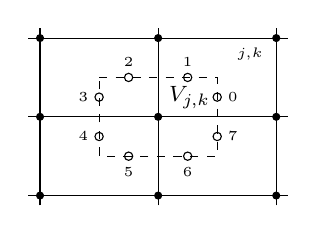
\begin{tikzpicture}[scale=0.5]
  % strong grid around elements
  \draw (-0.3,0) -- (6.3,0);
  \draw (-0.3,2) -- (6.3,2);
  \draw (-0.3,4) -- (6.3,4);
  \draw (0,-0.25) -- (0,4.25);
  \draw (3,-0.25) -- (3,4.25);
  \draw (6,-0.25) -- (6,4.25);
  % nodes
  \filldraw (0,0) circle (2.5pt);
  \filldraw (3,0) circle (2.5pt);
  \filldraw (6,0) circle (2.5pt);
  \filldraw (0,2) circle (2.5pt);
  \filldraw (3,2) circle (2.5pt);
  \filldraw (6,2) circle (2.5pt);
  \filldraw (0,4) circle (2.5pt);
  \filldraw (3,4) circle (2.5pt);
  \filldraw (6,4) circle (2.5pt);
  % outline control volume
  \draw[dashed] (1.5,3) -- (4.5,3) -- (4.5,1) -- (1.5,1) -- cycle;
  % mark quadrature points
  \draw (4.5,2.5) circle (3.0pt) node[shift={(0.2,0.0)}] {\tiny 0};
  \draw (3.75,3)  circle (3.0pt) node[shift={(0.0,0.2)}] {\tiny 1};
  \draw (2.25,3)  circle (3.0pt) node[shift={(0.0,0.2)}] {\tiny 2};
  \draw (1.5,2.5) circle (3.0pt) node[shift={(-0.2,0.0)}] {\tiny 3};
  \draw (1.5,1.5) circle (3.0pt) node[shift={(-0.2,0.0)}] {\tiny 4};
  \draw (2.25,1)  circle (3.0pt) node[shift={(0.0,-0.2)}] {\tiny 5};
  \draw (3.75,1)  circle (3.0pt) node[shift={(0.0,-0.2)}] {\tiny 6};
  \draw (4.5,1.5) circle (3.0pt) node[shift={(0.2,0.0)}] {\tiny 7};
  % label elements and control volume
  \draw (3.8,2.5) node {\footnotesize $V_{j,k}$};
  \draw (5.35,3.6) node {\scriptsize $\square_{j,k}$};
\end{tikzpicture}
\end{center}
  \item[$\circ$] these points good for any $\bq$, not just SIA
  \end{itemize}
\item a bit of upwinding improves convergence on non-flat beds
  \begin{itemize}
  \item[$\circ$] \dots even though this is a fully-implicit approach
  \item[$\circ$] tested on bedrock-step exact solution (Jarosch et al 2013)
  \item[$\circ$] details out of scope here
  \end{itemize}
\end{itemize}
\end{frame}


\begin{frame}{Newton's method, regularized}

\begin{itemize}
\item for $0 \le \eps \le 1$, regularize $\bq^{(\eps)}$
  \begin{itemize}
  \item[$\circ$] 12 levels: $\eps_0=1, \dots, \eps_{11}=2\times 10^{-4}, \eps_{12}=0$
  \item[$\circ$] $\bq^{(\eps_0)}$ with $\eps_0=1$ gives classical obstacle problem
    $$- \Div (D_0 \grad s) = a$$
  \item[$\circ$] $\bq^{(\eps_{12})}$ with $\eps_{12}=0$ gives SIA model
    $$- \Div (\Gamma h^{\nu+2} |\grad s|^{\nu-1} \grad s) = a$$
  \end{itemize}
\item at each level, use Newton's method
  \begin{itemize}
  \item[$\circ$] quadratic convergence for a dome test case:
  \end{itemize}
\end{itemize}

\begin{center}
\includegraphics[width=0.5\textwidth,keepaspectratio=true]{newtonconv}
\end{center}
\end{frame}


\section{results}

\begin{frame}{example: Greenland ice sheet}

\begin{columns}
\begin{column}{0.6\textwidth}
\begin{itemize}
\item \emph{goal}: given steady surface mass balance $a(x,y)$, and bedrock elevation $b(x,y)$, predict the thickness $h(x,y)$ of the Greenland ice sheet

\medskip
\item \emph{method} for steady SIA:
  \begin{itemize}
  \item[$\circ$] NCP form of \eqref{mc}
  \item[$\circ$] RS constrained-Newton
  \item[$\circ$] 900 m structured grid
  \item[$\circ$] $Q^1$ FEs in space
  \item[$\circ$] $N=7\times 10^6$ d.o.f.
  \end{itemize}

\medskip
\item \emph{result}: at right
  \begin{itemize}
  \item[$\circ$] see Bueler (2016), J.~Glaciol.
  \end{itemize}
\end{itemize}
\end{column}
\begin{column}{0.4\textwidth}
\vspace{-5mm}

\begin{center}
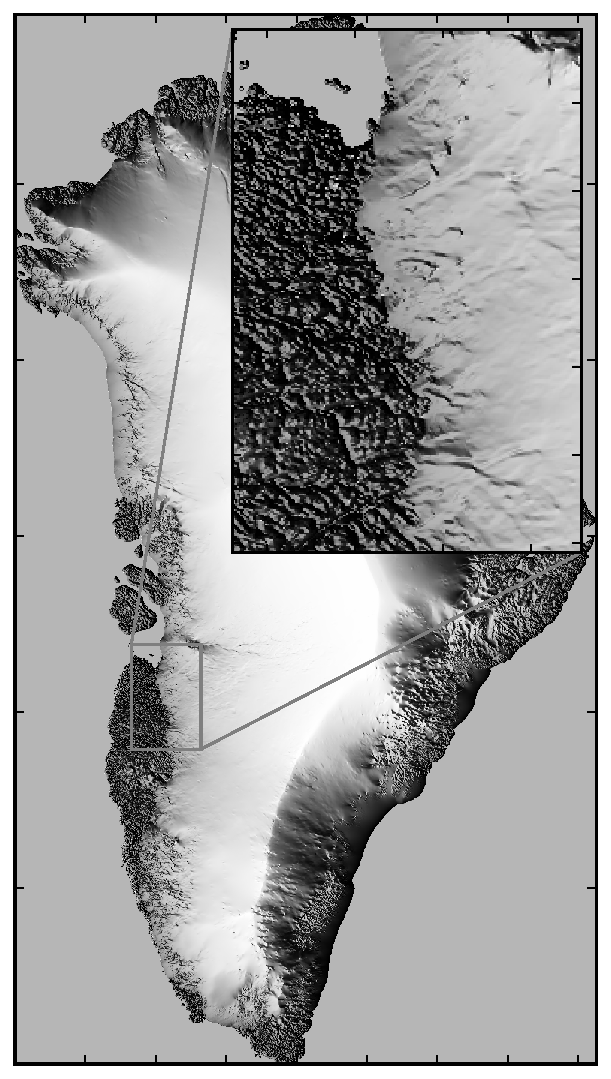
\includegraphics[width=0.95\textwidth,keepaspectratio=true]{grnwinset}
\end{center}
\end{column}
\end{columns}
\end{frame}


\begin{frame}{the essential difficulty: NASA's darn airplanes}

\begin{itemize}
\item actually: \alert{bedrock roughness}
\end{itemize}

\begin{columns}
\begin{column}{0.5\textwidth}
\hspace{10mm} \includegraphics[height=0.7\textheight,keepaspectratio=true]{scale-greenland-bed-old-oib}

\footnotesize \hspace{5mm} flight lines (OIB 2009-2014)
\end{column}
\begin{column}{0.6\textwidth}
\vspace{-8mm}

\hspace{10mm} \includegraphics[height=0.85\textheight,keepaspectratio=true]{scale-greenland-bed-mcb} 

\footnotesize result: Morlighem (2014) bed map
\end{column}
\end{columns}

\end{frame}


\begin{frame}{convergence consequences}

\begin{itemize}
\item improved observations $\implies$ worse solver convergence
  \begin{itemize}
  \item[$\circ$] old bed: Bamber (2001) on 5 km grid
  \item[$\circ$] new bed: Morlighem (2014) on 150 m grid
  \item[$\circ$] results shown for RS on NCP \eqref{mc}; SS is similar
  \end{itemize}
\end{itemize}

\begin{columns}
\begin{column}{0.4\textwidth}
\includegraphics[height=0.5\textheight,keepaspectratio=true]{insetinset}

rougher bed \hfill $\implies$ \phantom{sddf}
\end{column}
\begin{column}{0.6\textwidth}
\includegraphics[height=0.55\textheight,keepaspectratio=true]{rseps}

poorer Newton convergence
\end{column}
\end{columns}
\end{frame}


\section{conservation: failures and fixes}

\begin{frame}{my use of the word ``climate''}

\begin{itemize}
\item I have hijacked the word ``climate'' so as to define it to mean whatever I want
     \begin{itemize}
     \item[$\circ$] \emph{typical mathematician behavior} \dots
     \visible<2>{\item[$\circ$] you want a selfie? I'm not that kind of hijacker \dots}
     \end{itemize}

\bigskip
\item<2> my \emph{Definition}: for a fluid layer model, with governing weak formulation as above (and NCP/VI), the \emph{\alert{climate}} is the function $a(t,x,y,z)$ defined on the whole domain $\Omega$

\bigskip
\item<2> the climate is \emph{only} a source term in the PDE ``$h_t + \Div \bq = a$'' in those locations where $h>0$ (i.e.~$I_t$)
\item<2> we should be able to report how much mass was transferred to/from the fluid layer by the climate
\end{itemize}
\end{frame}


\begin{frame}{conservation reporting: subsets}
\begin{itemize}
\item back to time-stepping cases $\Delta t>0$
\item suppose $h^\ell$ solves the weak form \eqref{mc}
\item define
	\begin{align*}
	\Omega^\ell &= \left\{h^\ell(x,y) > 0\right\} \\
	\Omega^\ell_r &= \left\{h^\ell(x,y) = 0 \text{ and } h^{\ell-1}(x,y) > 0\right\} \quad \text{\alert{$\leftarrow$ retreat set}}
	\end{align*}
\end{itemize}

\vspace{-3mm}
\begin{center}
\includegraphics[width=0.8\textwidth,keepaspectratio=true]{cartoon-sets}
\end{center}
\end{frame}


\begin{frame}{conservation reporting: time-series}

\begin{itemize}
\item define:
   $$M^\ell = \int_\Omega h^\ell(x,y)\,dx\,dy, \qquad \text{\emph{the \alert{mass} (volume) at time} $t^\ell$}$$
\item then

\vspace{-8mm}
	\begin{align*}
	M^\ell - M^{\ell-1} &= \int_{\Omega^\ell} \mathLabelBox[
    labelstyle={xshift=1cm,yshift=2mm},
    linestyle={out=270,in=90, -latex}
    ]{h^\ell-h^{\ell-1}}{$\boxed{\Delta t\, (-\Div\bq^\ell + a^\ell)}$} \,dx\,dy + \int_{\Omega^\ell_r} 0 - h^{\ell-1} \,dx\,dy \\
	   &= \Delta t\, \left(0 + \int_{\Omega^\ell} a^\ell \,dx\,dy\right) - \int_{\Omega^\ell_r} h^{\ell-1} \,dx\,dy
	\end{align*}

	\begin{itemize}
\vspace{-1mm}
	\item[$\circ$] this assumes $\bq\to 0$ as $(x,y) \to \partial \Omega^\ell$
	\end{itemize}
\item new term:
     $$R^\ell = \int_{\Omega^\ell_r} h^{\ell-1} \,dx\,dy \qquad \text{the \emph{\alert{retreat loss} during step} $\ell$}$$
\end{itemize}
\end{frame}


\begin{frame}{conservation reporting: the limitation}

\begin{itemize}
\item \alert{the retreat loss $R^\ell$ is not balanced by the climate}
  \begin{itemize}
  \item[$\circ$] retreat $R^\ell$ is \emph{caused} by the climate, but we don't know a computable integral of $a^\ell$ to balance it
  \end{itemize}
\item we must track \alert{three} time series:
  \begin{itemize}
  \item[$\circ$] mass at time $t^\ell$: \qquad $M^\ell = \int_\Omega h^\ell(x,y)\,dx\,dy$

  \smallskip
  \item[$\circ$] climate over current fluid-covered region:
     $$C^\ell = \Delta t\, \int_{\Omega^\ell} a^\ell \,dx\,dy \qquad \approx \int_{t^{\ell-1}}^{t^\ell} \int_{I_t} a(t,x,y) \,dx\,dy\,dt$$
  \item[$\circ$] retreat loss during time step: \qquad $R^\ell = \int_{\Omega^\ell_r} h^{\ell-1} \,dx\,dy$
  \end{itemize}
\item and they balance:
     $$M^\ell = M^{\ell-1} + C^\ell - R^\ell$$
\end{itemize}
\end{frame}


\begin{frame}{conservation reporting: $R^\ell\to 0$ as $\Delta t \to 0$}

\begin{center}
\vspace{-3.3mm}

\animategraphics[autoplay,loop,height=2.9cm]{15}{../anim/tdep/u-}{1}{250}

\vspace{-1.1mm}
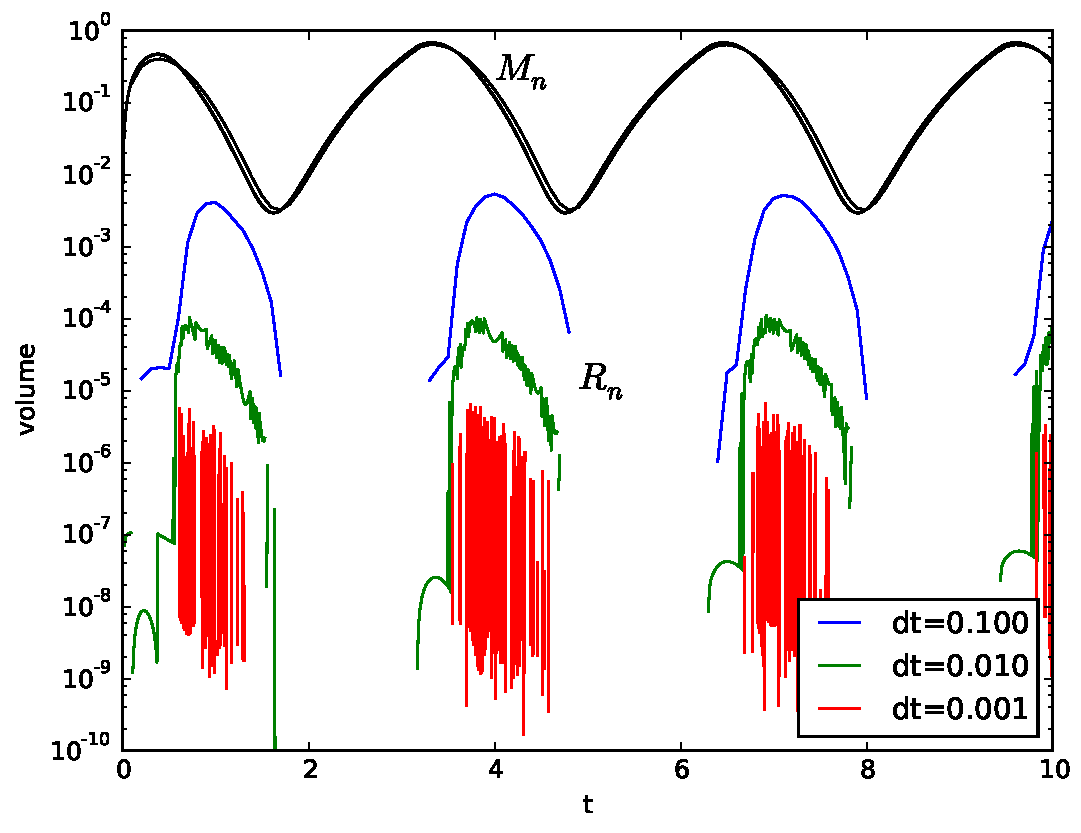
\includegraphics[width=0.64\textwidth,keepaspectratio=true]{masstimeseries} \, \phantom{!}
\end{center}
\end{frame}


\section{conclusion}

\begin{frame}{summary}

  \begin{itemize}
  \item \emph{problem}: fluid layer MC model \, ``$h_t + \Div\bq = a$''
    \begin{itemize}
    \item[$\circ$]  layer thickness $h$
    \item[$\circ$]  signed climate $a$
    \item[$\circ$]  coupled to momentum solver: $\bq=\bq(\bU,h)$
    \end{itemize}
  \item \emph{goals}:
    \begin{itemize}
    \item[$\circ$]  long (implicit) time steps
    \item[$\circ$]  rigorous conservation reporting
    \end{itemize}
  \item \emph{approach}:
    \begin{itemize}
    \item[$\circ$]  pose single time-step problem weakly as NCP or VI
      \begin{itemize}
      \item  incorporates constraint $h\ge 0$
      \item  approach is $\bq$-agnostic
      \end{itemize}
    \item[$\circ$]  solve by scalable constrained-Newton method (e.g.~PETSc)
    \end{itemize}
  \item \emph{challenges}:
    \begin{itemize}
    \item[$\circ$]  bed roughness makes convergence hard
    \item[$\circ$]  can this lead to global glaciation modeling?
    \end{itemize}
  \end{itemize}
\end{frame}



\end{document}
